\section{308 --- Range Sum Query 2D - Mutable}
Given a 2D matrix matrix $M$, find the sum of the elements inside the rectangle defined by its upper left corner $(r_1, c_1)$ and lower right corner $(r_2, c_2)$.
\begin{figure}[H]
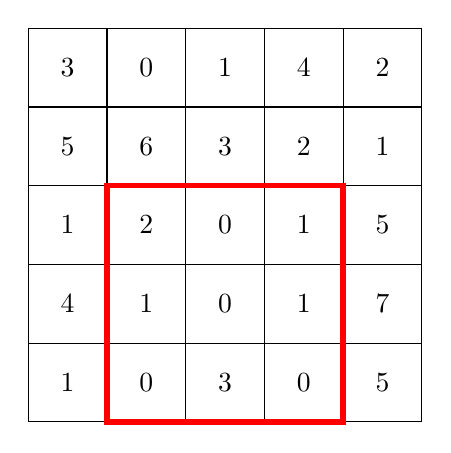
\begin{tikzpicture}
\draw[black, thin] (0,0) grid (5,5);
\node at (0.5,4.5) {$3$};
\node at (1.5,4.5) {$0$};
\node at (2.5,4.5) {$1$};
\node at (3.5,4.5) {$4$};
\node at (4.5,4.5) {$2$};
%row2
\node at (0.5,3.5) {$5$};
\node at (1.5,3.5) {$6$};
\node at (2.5,3.5) {$3$};
\node at (3.5,3.5) {$2$};
\node at (4.5,3.5) {$1$};
%row3
\node at (0.5,2.5) {$1$};
\node at (1.5,2.5) {$2$};
\node at (2.5,2.5) {$0$};
\node at (3.5,2.5) {$1$};
\node at (4.5,2.5) {$5$};
%row 4
\node at (0.5,1.5) {$4$};
\node at (1.5,1.5) {$1$};
\node at (2.5,1.5) {$0$};
\node at (3.5,1.5) {$1$};
\node at (4.5,1.5) {$7$};
%row 5
\node at (0.5,0.5) {$1$};
\node at (1.5,0.5) {$0$};
\node at (2.5,0.5) {$3$};
\node at (3.5,0.5) {$0$};
\node at (4.5,0.5) {$5$};
\draw[line width=2pt,red] (1,0) rectangle ++(3,3);
\end{tikzpicture}
\end{figure}
The above rectangle (with the red border) is defined by $(r_1, c_1) = (2, 1)$ and $(r_2, c_2) = (4, 3)$, which contains sum = 8.
\paragraph{Example:}
\begin{flushleft}
Give matrix $M$ is
\begin{table}[H]
    \begin{tabular}{ccccc}
        3 & 0 & 1 & 4 & 2 \\
        5 &  6 &  3 &  2 &  1\\
        1 &  2 &  0 &  1 &  5 \\
        4 &  1 &  0 &  1 &  7\\
        1 &  0 &  3 &  0 &  5
    \end{tabular}
\end{table}
\begin{lstlisting}[style=customc]
sumRegion(2, 1, 4, 3); // 8
update(3, 2, 2);
sumRegion(2, 1, 4, 3); // 10
\end{lstlisting}
\end{flushleft}

\paragraph{Note:}
\begin{itemize}
\item The matrix is only modifiable by the update function.
\item You may assume the number of calls to \texttt{update} and \texttt{sumRegion} function is distributed evenly.
 \item You may assume that $r_1 \leq r_2$ and $c_1 \leq c_2$.
\end{itemize}
\subsection{2D BIT}
\begin{itemize}
\item 为了快速update 二维区域,还是采用BIT的数据结构,但是是2D,即row和column分别按照BIT进行build。算法和一维的没有区别。
\item 与1维的BIT类似, 2D BIT也是只能得到从$ (0,0) $到 $ (r,c) $的区间和,因此需要按照304中的分区域计算方法,分别计算出四个角的区域和。
\item 如果$M$的dimension为$m\times n$,与1维的BIT类似,2维的BIT的dimension is equal to $ (m+1)\times (n+1) $
\end{itemize}
\setcounter{lstlisting}{0}
\begin{lstlisting}[style=customc, caption={BIT}]
class NumMatrix
{
public:
    NumMatrix( vector<vector<int>> &matrix )
        : M( matrix )
    {
        vector<vector<int>> tmp( M.size() + 1, vector<int> ( M[0].size() + 1, 0 ) );

        swap( tmp, BIT );

        m = static_cast< int >( M.size() );
        n = static_cast< int >( M[0].size() );

        for( int r = 0; r < m; ++r )
        {
            for( int c = 0; c < n; ++c )
            {
                updateBIT( r, c, M[r][c] );
            }
        }
    }

    void update( int row, int col, int val )
    {
        int diff = val - M[row][col];

        updateBIT( row, col, diff );
    }

    int sumRegion( int row1, int col1, int row2, int col2 )
    {
        //Four regions computation
        return sumBIT( row2, col2 )
               - sumBIT( row1 - 1, col2 )
               - sumBIT( row2, col1 - 1 )
               + sumBIT( row1 - 1, col1 - 1 );
    }

private:

    void updateBIT( int r, int c, int diff )
    {
        int x = r + 1;

        while( x <= m )
        {
            //must reset y at each iteration
            int y = c + 1;

            while( y <= n )
            {
                BIT[x][y] += diff;

                y += ( y & ( -y ) );
            }

            x += ( x & ( -x ) );
        }
    }

    int sumBIT( int r, int c )
    {
        int x = r + 1;

        int sum = 0;

        while( x > 0 )
        {
            //must reset y at each iteration
            int y = c + 1;

            while( y > 0 )
            {
                sum += BIT[x][y];
                y -= ( y & ( -y ) );
            }

            x -= ( x & ( -x ) );
        }

        return sum;
    }

    vector<vector<int>>& M;
    vector<vector<int>> BIT;

    int m;
    int n;
};
\end{lstlisting}